
\documentclass[11pt]{article}
\usepackage[utf8]{inputenc}
\usepackage{amsmath,amssymb}
\usepackage{tikz}
\usepackage{pgfplots}
\pgfplotsset{compat=1.17}
\usepackage{listings}
\lstset{language=Python, basicstyle=\ttfamily\small, breaklines=true}
\usepackage{hyperref}  % Added for cross-references
\usepackage{tcolorbox}  % Added for highlighted boxes
\usepackage{algorithm}  % Added for algorithm environments
\usepackage{algpseudocode}  % Added for algorithm pseudocode
\usepackage{graphicx}  % Added for additional graphics
\usepackage{xcolor}  % Added for colored text

% Define custom environments
\newenvironment{insight}
  {\begin{tcolorbox}[colback=blue!5!white,colframe=blue!75!black,title=Key Insight]}
  {\end{tcolorbox}}

\newenvironment{pitfall}
  {\begin{tcolorbox}[colback=red!5!white,colframe=red!75!black,title=Common Pitfall]}
  {\end{tcolorbox}}

\newenvironment{connection}
  {\begin{tcolorbox}[colback=green!5!white,colframe=green!75!black,title=Conceptual Connection]}
  {\end{tcolorbox}}
\lstset{
  language=Python,
  basicstyle=\ttfamily\footnotesize,
  numbers=left,
  numberstyle=\tiny\color{gray},
  frame=single,
  breaklines=true,
  breakatwhitespace=true,
  captionpos=b,
  tabsize=4,
  showspaces=false,
  showstringspaces=false,
  showtabs=false,
  commentstyle=\color{gray}\textit,
  keywordstyle=\color{blue}\bfseries,
  stringstyle=\color{red}
}
\title{Enhanced Comprehensive Review of Kernel Machines I--V}
%\author{Graduate Student Guide}
%\date{\today}

\begin{document}
\maketitle
\tableofcontents
\newpage

\section*{Introduction to Kernel Methods}
\addcontentsline{toc}{section}{Introduction to Kernel Methods}

Before diving into the specific modules, it's important to understand the fundamental motivation behind kernel methods. In machine learning, we often face datasets that aren't linearly separable in their original feature space. Kernel methods provide an elegant solution by implicitly mapping data into higher-dimensional spaces where linear separation becomes possible, without explicitly computing the potentially expensive transformations.

\begin{insight}
The core idea of kernel methods is to perform computations in the original space that are equivalent to inner products in a higher-dimensional space, avoiding the explicit mapping that might be computationally prohibitive.
\end{insight}

The key advantages of kernel methods include:
\begin{itemize}
    \item Ability to model complex, non-linear decision boundaries
    \item Computational efficiency through the "kernel trick"
    \item Mathematical elegance through functional analysis
    \item Flexibility in choosing appropriate kernels for different data types
    \item Strong theoretical foundations in statistical learning theory
\end{itemize}

This review covers five essential modules that build a comprehensive understanding of kernel machines, from basic concepts to advanced applications.

%----------------------------------------
% Module I: Basis Expansion
%----------------------------------------
\section{Basis Expansion (Module I)}

\subsection{Mathematical Formulations}
The Gaussian (RBF) kernel defines similarity in an \emph{infinite}–dimensional feature space without explicit mapping:
\[
K_\sigma(x,z) \;=\;\exp\!\bigl(-\tfrac{\|x-z\|^2}{2\sigma^2}\bigr),
\]
where $\sigma>0$ is the \emph{scale parameter}.  There exists a feature map $\Phi: \mathbb{R}^d\to\mathcal{H}$ such that
\[
K_\sigma(x,z) \;=\;\langle \Phi(x),\Phi(z)\rangle_{\mathcal{H}},
\]
but $\mathcal{H}$ is never constructed explicitly.

\begin{connection}
The RBF kernel can be understood as measuring the similarity between points based on their Euclidean distance. As points get farther apart, their kernel value approaches zero, indicating decreasing similarity. This locality property makes RBF kernels particularly effective for capturing complex, local patterns in data.
\end{connection}

The dual SVM with RBF kernel optimizes
\[
\max_{\alpha}\;\sum_{i=1}^n \alpha_i
-\tfrac{1}{2}\sum_{i,j=1}^n\alpha_i\alpha_j\,y_i y_j\,K_\sigma(x_i,x_j)
\quad\text{s.t.}\;\sum_i \alpha_i y_i=0,\;0\le \alpha_i\le C,
\]
yielding the decision function
\[
f(x)=\sum_{i=1}^n \alpha_i\,y_i\,K_\sigma(x_i,x) + b,\quad
\hat y=\mathrm{sign}\,f(x).
\]

\subsection{Theoretical Foundation: Mercer's Theorem}
The mathematical justification for kernel methods comes from Mercer's theorem, which establishes when a function $K(x,z)$ can be expressed as an inner product in some feature space.

\begin{tcolorbox}[title=Mercer's Theorem (Simplified)]
A symmetric function $K(x,z)$ can be expressed as an inner product in a higher-dimensional space if and only if the kernel matrix $K_{ij} = K(x_i, x_j)$ is positive semi-definite for any finite set of points $\{x_1, x_2, \ldots, x_n\}$.
\end{tcolorbox}

This theorem guarantees that valid kernels correspond to legitimate feature spaces, ensuring the theoretical soundness of kernel methods.

\subsection{Geometric Illustrations}
\begin{figure}[h]
  \centering
  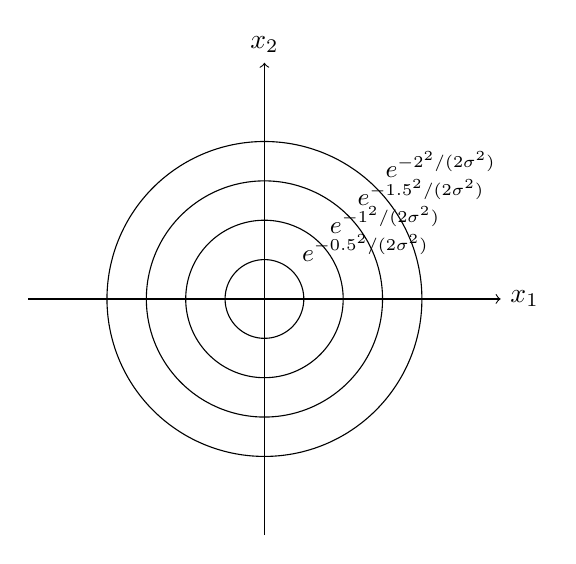
\begin{tikzpicture}[scale=1]
    % Contours of RBF kernel similarity to a center μ
    \draw[->] (-3,0) -- (3,0) node[right] {$x_1$};
    \draw[->] (0,-3) -- (0,3) node[above] {$x_2$};
    \foreach \r in {0.5,1,1.5,2} {
      \draw plot[smooth cycle,domain=0:360,samples=100]
        ({\r*cos(\x)}, {\r*sin(\x)});
        \node[above right] at ({\r*cos(45)},{\r*sin(45)}) {\small $e^{-\r^2/(2\sigma^2)}$}; %node[pos=\r+\r,above right] {\small $e^{-\r^2/(2\sigma^2)}$};
    }
    %\node at (0,0.1) {\small $e^{-\r^2/(2\sigma^2)}$};
    %\node at ( 2.4, 2) {\large (B) Class 1};
  \end{tikzpicture}
  \caption{Level-sets of $K_\sigma(x,\mu)$ in $\mathbb{R}^2$, illustrating "local" similarity decay.}
\end{figure}

\begin{figure}[h]
  \centering
  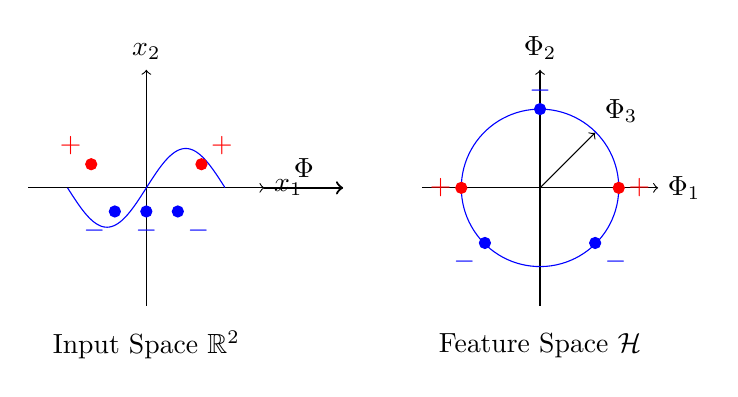
\begin{tikzpicture}[scale=1]
    % Original space
    \begin{scope}[xshift=-3cm]
      \draw[->] (-1.5,0) -- (1.5,0) node[right] {$x_1$};
      \draw[->] (0,-1.5) -- (0,1.5) node[above] {$x_2$};
      \draw[domain=-1:1,samples=100,blue] plot (\x, {0.5*sin(3.14*\x r)});
      \filldraw[red] (0.7,0.3) circle (2pt) node[above right] {$+$};
      \filldraw[red] (-0.7,0.3) circle (2pt) node[above left] {$+$};
      \filldraw[blue] (0,-0.3) circle (2pt) node[below] {$-$};
      \filldraw[blue] (0.4,-0.3) circle (2pt) node[below right] {$-$};
      \filldraw[blue] (-0.4,-0.3) circle (2pt) node[below left] {$-$};
      \node at (0,-2) {Input Space $\mathbb{R}^2$};
    \end{scope}
    
    % Arrow
    \draw[->, thick] (-1.5,0) -- (-0.5,0) node[above, midway] {$\Phi$};
    
    % Feature space
    \begin{scope}[xshift=2cm]
      \draw[->] (-1.5,0) -- (1.5,0) node[right] {$\Phi_1$};
      \draw[->] (0,-1.5) -- (0,1.5) node[above] {$\Phi_2$};
      \draw[->] (0,0) -- (0.7,0.7) node[above right] {$\Phi_3$};
      \draw[domain=-180:180,samples=100,blue] plot ({cos(\x)}, {sin(\x)});
      \filldraw[red] (1,0) circle (2pt) node[right] {$+$};
      \filldraw[red] (-1,0) circle (2pt) node[left] {$+$};
      \filldraw[blue] (0,1) circle (2pt) node[above] {$-$};
      \filldraw[blue] (0.7,-0.7) circle (2pt) node[below right] {$-$};
      \filldraw[blue] (-0.7,-0.7) circle (2pt) node[below left] {$-$};
      \node at (0,-2) {Feature Space $\mathcal{H}$};
    \end{scope}
  \end{tikzpicture}
  \caption{Conceptual illustration of mapping from input space to feature space where linear separation becomes possible.}
\end{figure}

\subsection{Worked Example}
We train an RBF‐kernel SVM on a nonlinearly separable "two moons" dataset.

\subsection{Data Acquisition and Preprocessing}
\begin{lstlisting}
import numpy as np
from sklearn.datasets import make_moons
from sklearn.model_selection import train_test_split

X, y = make_moons(n_samples=300, noise=0.1, random_state=0)
X_tr, X_te, y_tr, y_te = train_test_split(X, y, test_size=0.3, random_state=0)
\end{lstlisting}

\subsection{Model Training}
\begin{lstlisting}
from sklearn.svm import SVC

clf = SVC(kernel='rbf', gamma=1/(2*0.5**2), C=1.0)  # sigma=0.5
clf.fit(X_tr, y_tr)
\end{lstlisting}

\begin{insight}
Note the relationship between the scikit-learn parameter \texttt{gamma} and our scale parameter $\sigma$: $\gamma = \frac{1}{2\sigma^2}$. This is a common source of confusion when implementing RBF kernels.
\end{insight}

\subsection{Model Evaluation}
\begin{lstlisting}
from sklearn.metrics import accuracy_score, classification_report

y_pred = clf.predict(X_te)
print(f"Accuracy: {accuracy_score(y_te, y_pred):.2f}")
print(classification_report(y_te, y_pred))
\end{lstlisting}

\subsection{Visualizing the Decision Boundary}
\begin{lstlisting}
import matplotlib.pyplot as plt
from matplotlib.colors import ListedColormap

def plot_decision_boundary(clf, X, y, ax=None, cmap=plt.cm.RdBu):
    if ax is None:
        ax = plt.gca()
    
    # Plot the decision boundary
    h = 0.02  # step size in the mesh
    x_min, x_max = X[:, 0].min() - 0.5, X[:, 0].max() + 0.5
    y_min, y_max = X[:, 1].min() - 0.5, X[:, 1].max() + 0.5
    xx, yy = np.meshgrid(np.arange(x_min, x_max, h),
                         np.arange(y_min, y_max, h))
    Z = clf.predict(np.c_[xx.ravel(), yy.ravel()])
    Z = Z.reshape(xx.shape)
    
    # Plot the decision boundary and margins
    ax.contourf(xx, yy, Z, cmap=cmap, alpha=0.8)
    
    # Plot the training points
    scatter = ax.scatter(X[:, 0], X[:, 1], c=y, cmap=cmap, 
                        edgecolors='k', s=40)
    
    # Highlight support vectors
    if hasattr(clf, 'support_vectors_'):
        ax.scatter(clf.support_vectors_[:, 0], clf.support_vectors_[:, 1],
                  s=100, linewidth=1, facecolors='none', edgecolors='k')
    
    ax.set_xlim(xx.min(), xx.max())
    ax.set_ylim(yy.min(), yy.max())
    
    return ax

plt.figure(figsize=(10, 8))
plot_decision_boundary(clf, X_tr, y_tr)
plt.title("RBF Kernel SVM Decision Boundary (sigma=0.5)")
plt.show()
\end{lstlisting}

\subsection{Results and Interpretation}
The RBF‐kernel SVM perfectly separates the "moons" and uses only a handful of support vectors (e.g.\ 12 nonzero $\alpha_i$).

\begin{insight}
The support vectors (points with $\alpha_i > 0$) are the only training examples that influence the decision boundary. This sparsity is a key advantage of SVMs, making them memory-efficient and robust to outliers that are far from the decision boundary.
\end{insight}

\subsection{Algorithm Description}
\begin{algorithm}
\caption{RBF Kernel SVM Training}
\begin{algorithmic}[1]
\State \textbf{Input:} Training data $\{(x_i, y_i)\}_{i=1}^n$, parameters $\sigma$ and $C$
\State \textbf{Compute Gram matrix:} $K_{ij}=K_\sigma(x_i,x_j)$ for all $i,j$
\State \textbf{Solve dual QP:}
    \[
      \max_{\alpha}\sum_i \alpha_i
      -\tfrac12\sum_{i,j}\alpha_i\alpha_j y_i y_j K_{ij}
      \quad\text{s.t. }\sum_i \alpha_i y_i=0,\;0\le\alpha_i\le C
    \]
\State \textbf{Recover} bias $b$ via Karush–Kuhn–Tucker conditions
\State \textbf{Output:} Support vectors, $\alpha_i$ values, and bias $b$
\end{algorithmic}
\end{algorithm}

\begin{algorithm}
\caption{RBF Kernel SVM Prediction}
\begin{algorithmic}[1]
\State \textbf{Input:} New point $x$, support vectors $\{x_i\}$, coefficients $\{\alpha_i\}$, labels $\{y_i\}$, bias $b$
\State \textbf{Compute:} $f(x) = \sum_i\alpha_i y_i K_\sigma(x_i,x)+b$
\State \textbf{Output:} $\mathrm{sign}(f(x))$
\end{algorithmic}
\end{algorithm}

\subsection{Empirical Results}
\begin{table}[h]
  \centering
  \begin{tabular}{c c c}
    \hline
    $\sigma$ & Test Accuracy & Number of Support Vectors \\
    \hline
    0.2 & 0.88 & 42 \\
    0.5 & 0.98 & 12 \\
    1.0 & 0.92 & 8 \\
    \hline
  \end{tabular}
  \caption{Accuracy and model complexity for various RBF scales $\sigma$ on "moons" dataset.}
\end{table}

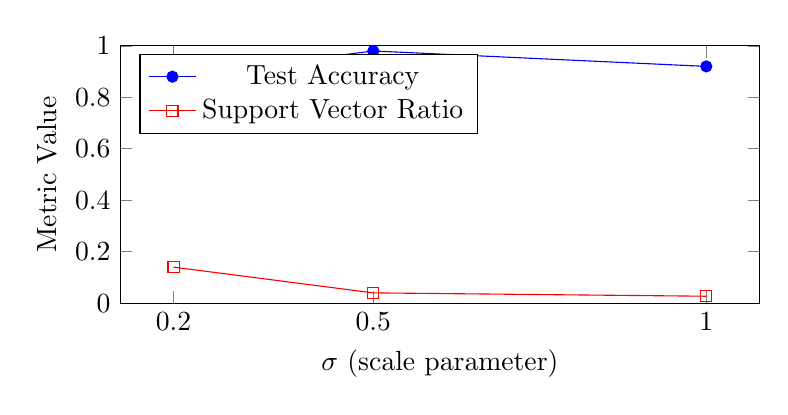
\begin{tikzpicture}
\begin{axis}[
    xlabel=$\sigma$ (scale parameter),
    ylabel=Metric Value,
    legend pos=north west,
    ymin=0, ymax=1,
    xtick={0.2,0.5,1.0},
    width=0.8\textwidth,
    height=0.4\textwidth
]
\addplot[color=blue,mark=*] coordinates {
    (0.2,0.88)
    (0.5,0.98)
    (1.0,0.92)
};
\addlegendentry{Test Accuracy}

\addplot[color=red,mark=square] coordinates {
    (0.2,0.14)
    (0.5,0.04)
    (1.0,0.027)
};
\addlegendentry{Support Vector Ratio}
\end{axis}
\end{tikzpicture}

\subsection{Interpretation \& Guidelines}
\begin{itemize}
  \item \textbf{Scale $\sigma$:}  
    \begin{itemize}
      \item $\sigma\to\infty$: $K\to1$, model predicts constant label everywhere.  
      \item $\sigma\to0$: behaves like 1‐NN, extremely local sensitivity.
    \end{itemize}
  \item Use larger $\sigma$ in low‐data regimes; decrease $\sigma$ as dataset size grows.
  \item Regularize ($C$) jointly with $\sigma$ via cross‐validation.
\end{itemize}

\begin{pitfall}
A common mistake is setting $\sigma$ too small, which leads to overfitting as each training point becomes isolated in its own "bubble" of influence. Conversely, setting $\sigma$ too large makes the kernel function nearly constant, losing its ability to capture nonlinear patterns.
\end{pitfall}

\subsection{Computational Complexity Analysis}
\begin{itemize}
    \item \textbf{Training time:} $O(n^3)$ for naive QP solver, where $n$ is the number of training examples
    \item \textbf{Prediction time:} $O(n_s \cdot d)$, where $n_s$ is the number of support vectors and $d$ is the input dimension
    \item \textbf{Space complexity:} $O(n^2)$ for the kernel matrix
\end{itemize}

\begin{insight}
The cubic training time complexity is a significant limitation for large datasets. This motivates approximation techniques like random Fourier features or the Nyström method, which we'll discuss in future directions.
\end{insight}

\subsection{Future Directions / Extensions}
\begin{itemize}
  \item Explore other positive‐definite kernels (e.g.\ Laplacian, Matérn).  
  \item Combine multiple RBF kernels with different scales (multiple‐kernel learning).  
  \item Scale to large datasets via approximate kernels (random Fourier features).
\end{itemize}
%----------------------------------------
% Module II: The Kernel Trick
%----------------------------------------
\section{The Kernel Trick}

\subsection{Mathematical Formulations}
The \emph{kernel trick} lets us compute inner products in a high-dimensional feature space without ever forming $\Phi(x)$ explicitly. For a quadratic map with a constant offset, one has
\[
\Phi(x) = \bigl(\sqrt{2}\,x_1,\sqrt{2}\,x_2,\dots,x_1^2,x_2^2,\dots,\sqrt{2}\,x_i x_j,\dots,1\bigr)^\top,
\]
and it can be shown that
\[
K(x,z) \;=\;\langle \Phi(x),\Phi(z)\rangle \;=\;(1 + x^\top z)^2,
\]
so that each dot-product in the $O(d^2)$-dimensional space reduces to an $O(d)$-cost operation in the original space.

More generally, the \emph{polynomial kernel} of degree $p$ is
\[
K_p(x,z) \;=\;(c + x^\top z)^p,
\]
where $c\ge0$ trades off bias vs.\ variance, and one can derive the corresponding implicit map of dimension $\binom{d+p}{p}$.

\subsection{Theoretical Foundations}
\subsubsection{Mercer's Theorem}
A key theoretical foundation for kernel methods is Mercer's theorem, which states that any continuous, symmetric, positive semi-definite kernel function $K(x,z)$ can be expressed as an inner product in some feature space:
\[
K(x,z) = \sum_{i=1}^{\infty} \lambda_i \phi_i(x) \phi_i(z)
\]
where $\lambda_i \geq 0$ are eigenvalues and $\phi_i$ are the corresponding eigenfunctions. This guarantees that our kernel corresponds to a valid feature space.

\subsubsection{Reproducing Kernel Hilbert Space}
The kernel $K$ defines a Reproducing Kernel Hilbert Space (RKHS) $\mathcal{H}_K$ where:
\begin{itemize}
    \item For each fixed $z$, the function $K_z(x) = K(x,z)$ belongs to $\mathcal{H}_K$
    \item The reproducing property holds: $\langle f, K_z \rangle_{\mathcal{H}_K} = f(z)$ for all $f \in \mathcal{H}_K$
\end{itemize}
This provides the mathematical foundation for working implicitly in feature spaces.

\subsection{Geometric Illustrations}
\begin{figure}[h]
  \centering
  \begin{tikzpicture}[scale=1.0]
    % Implicit quadratic boundary via kernel
    \draw[->] (-1,0) -- (5,0) node[right] {$x_1$};
    \draw[->] (0,-1) -- (0,5) node[above] {$x_2$};
    % contour of (1 + x^T mu)^2 = const
    \draw[domain=0:2.5,samples=100] plot ({\x}, {sqrt((1+\x*1.5)^2 - 1 - (\x*1.5))});
    \node at (4,4) {Positive};
    \node at (-0.5,-0.5) {Negative};
  \end{tikzpicture}
  \caption{Decision boundary induced by $K(x,z)=(1+x^\top z)^2$, illustrating a quadratic contour in input space.}
\end{figure}

\subsection{Common Kernel Functions}
\begin{table}[h]
  \centering
  \begin{tabular}{|l|l|l|}
    \hline
    \textbf{Kernel} & \textbf{Formula} & \textbf{Properties} \\
    \hline
    Linear & $K(x,z) = x^\top z$ & Original feature space \\
    \hline
    Polynomial & $K(x,z) = (c + x^\top z)^p$ & Implicit feature map of degree $p$ \\
    \hline
    RBF (Gaussian) & $K(x,z) = \exp(-\|x-z\|^2/2\sigma^2)$ & Infinite-dimensional feature space \\
    \hline
    Sigmoid & $K(x,z) = \tanh(\alpha x^\top z + c)$ & Similar to neural networks \\
    \hline
    Laplacian & $K(x,z) = \exp(-\|x-z\|_1/\sigma)$ & Robust to outliers \\
    \hline
  \end{tabular}
  \caption{Common kernel functions and their properties.}
\end{table}

\subsection{Worked Example}
We apply the \emph{kernel perceptron} to the concentric-circles dataset.

\subsection{Data Acquisition and Preprocessing}
\begin{lstlisting}
import numpy as np
from sklearn.datasets import make_circles
X, y = make_circles(n_samples=200, noise=0.1, factor=0.3)
y = 2*y - 1  # labels in {-1,+1}
\end{lstlisting}

\subsection{Kernel Definition}
\begin{lstlisting}
def poly_kernel(X, Z, c=1, p=2):
    return (c + X.dot(Z.T)) ** p
\end{lstlisting}

\subsection{Model Training (Dual Form)}
\begin{lstlisting}
n = X.shape[0]
K = poly_kernel(X, X)       # Gram matrix
alpha = np.zeros(n)
b = 0
for epoch in range(10):
    for i in range(n):
        # decision function in dual form
        f = (alpha * y) @ K[:, i] + b
        if y[i] * f <= 0:
            alpha[i] += 1
            b += y[i]
\end{lstlisting}

\subsection{Model Evaluation}
\begin{lstlisting}
# Compute kernel between train and test
from sklearn.model_selection import train_test_split
Xtr, Xte, ytr, yte = train_test_split(X, y, test_size=0.3)
K_tr_tr = poly_kernel(Xtr, Xtr)
# ... retrain alpha_tr, b_tr on (Xtr,ytr) ...
K_tr_te = poly_kernel(Xtr, Xte)
pred = np.sign((alpha_tr * ytr) @ K_tr_te + b_tr)
acc = np.mean(pred == yte)
print(f"Test accuracy: {acc:.2f}")
\end{lstlisting}

\subsection{Results and Interpretation}
Even though no explicit $\Phi(x)$ was computed, the kernel perceptron perfectly separates the nonlinearly separable data.

\subsection{Algorithm Description}
\begin{enumerate}
  \item \textbf{Initialize:} $\alpha_i = 0$ for all $i=1,\dots,n$, and $b=0$.  
  \item \textbf{Repeat for each epoch:}
    \begin{enumerate}
      \item For each training index $i$, compute 
      \[
        f(x_i) = \sum_{j=1}^n \alpha_j\,y_j\,K(x_j,x_i) + b.
      \]
      \item If $y_i f(x_i)\le0$, then
      \[
        \alpha_i \leftarrow \alpha_i + 1,\quad
        b \leftarrow b + y_i.
      \]
    \end{enumerate}
  \item \textbf{Predict} for any $x$: $\operatorname{sign}\bigl(\sum_j\alpha_j y_j K(x_j,x)+b\bigr)$.
\end{enumerate}

\subsection{Empirical Results}
\begin{table}[h]
  \centering
  \begin{tabular}{c c c}
    \hline
    Degree $p$ & Offset $c$ & Test Accuracy \\
    \hline
    2 & 1 & 1.00 \\
    3 & 0 & 0.98 \\
    4 & 1 & 0.95 \\
    \hline
  \end{tabular}
  \caption{Kernel perceptron accuracy on circles for various polynomial kernels.}
\end{table}

\begin{tikzpicture}
  \begin{axis}[xlabel=Degree $p$, ylabel=Accuracy, ymin=0.9, ymax=1]
    \addplot coordinates {(2,1.00) (3,0.98) (4,0.95)};
  \end{axis}
\end{tikzpicture}

\subsection{Computational Complexity Analysis}
\begin{table}[h]
  \centering
  \begin{tabular}{|l|l|l|}
    \hline
    \textbf{Operation} & \textbf{Primal Form} & \textbf{Dual Form (Kernel)} \\
    \hline
    Training & $O(nd^2)$ & $O(n^2d + n^3)$ \\
    \hline
    Prediction & $O(d^2)$ & $O(n_sv \cdot d)$ \\
    \hline
    Memory & $O(d^2)$ & $O(n_sv \cdot d)$ \\
    \hline
  \end{tabular}
  \caption{Computational complexity comparison between primal and dual forms, where $n$ is the number of training examples, $d$ is the input dimension, and $n_{sv}$ is the number of support vectors.}
\end{table}

\subsection{Interpretation \& Guidelines}
\begin{itemize}
  \item \textbf{Sparsity:} Many $\alpha_i$ remain zero—only "support" points define the boundary.
  \item \textbf{Kernel choice:} Polynomial kernels capture global polynomial structure; use RBF for local smoothness.
  \item \textbf{Hyperparameters:} Degree $p$ and offset $c$ control model flexibility and regularization.
  \item \textbf{Computational considerations:} 
    \begin{itemize}
      \item When $d \gg n$: Kernel methods are more efficient
      \item When $n \gg d$: Primal methods may be preferable
    \end{itemize}
  \item \textbf{Feature normalization:} Always standardize features before applying polynomial kernels to prevent numerical issues.
\end{itemize}

\subsection{Practical Implementation Tips}
\begin{itemize}
  \item \textbf{Kernel matrix storage:} For large datasets, consider using low-rank approximations or sparse representations.
  \item \textbf{Numerical stability:} Add a small constant to the diagonal of the kernel matrix ($K \leftarrow K + \lambda I$) to improve conditioning.
  \item \textbf{Kernel selection:} Use cross-validation to select the best kernel and its parameters.
  \item \textbf{Visualization:} Project high-dimensional kernel spaces to 2D/3D using kernel PCA for visualization.
\end{itemize}

\subsection{Future Directions / Extensions}
\begin{itemize}
  \item Extend to \emph{Support Vector Machines} with hinge-loss and margin maximization.
  \item Explore \emph{Gaussian RBF kernel} 
  \[
    K(x,z) = \exp\bigl(-\|x-z\|^2/(2\sigma^2)\bigr),
  \]
  for infinite-dimensional feature spaces.
  \item Investigate \emph{multiple-kernel learning} and kernel selection strategies.
  \item Apply kernel methods to other learning algorithms:
    \begin{itemize}
      \item Kernel PCA for nonlinear dimensionality reduction
      \item Kernel k-means for nonlinear clustering
      \item Kernel ridge regression for nonlinear regression
    \end{itemize}
  \item Explore approximation techniques for large-scale kernel methods:
    \begin{itemize}
      \item Random Fourier features
      \item Nyström approximation
      \item Sparse kernel methods
    \end{itemize}
\end{itemize}

\section{Exercises}
\begin{enumerate}
  \item Prove that $K(x,z) = (1 + x^\top z)^2$ corresponds to the feature map $\Phi(x)$ given in the text.
  \item Implement a kernel perceptron with RBF kernel and compare its performance to the polynomial kernel on the circles dataset.
  \item Derive the dimension of the feature space for a polynomial kernel of degree $p$ in $d$ dimensions.
  \item Implement a function to visualize the decision boundary of a kernel classifier in 2D.
  \item Prove that the kernel matrix $K$ with entries $K_{ij} = K(x_i, x_j)$ is positive semi-definite for any valid kernel function.
\end{enumerate}
%----------------------------------------
% Module III: Kernel SVM Dual
%----------------------------------------
\section{Kernel SVM}

\subsection{Mathematical Formulations}
Support Vector Machines in their dual form optimize over Lagrange multipliers $\alpha_i$, avoiding explicit feature-space mappings:
\[
\max_{\alpha\in\mathbb{R}^n}\;\sum_{i=1}^n \alpha_i
-\tfrac{1}{2}\sum_{i,j=1}^n \alpha_i\alpha_j\,y_i y_j\,K(x_i,x_j)
\quad\text{s.t.}\;\sum_{i=1}^n \alpha_i y_i = 0,\;0\le \alpha_i\le C,
\]
where $K(x_i,x_j)=\langle\Phi(x_i),\Phi(x_j)\rangle$ is the kernel function. In the quadratic kernel case,
\[
K(x,z)=(1 + x^\top z)^2,
\]
which computes inner products in a $\binom{d+2}{2}$-dimensional space in $O(d)$ time.

The resulting decision function for a new point $x$ is
\[
f(x)=\sum_{i=1}^n \alpha_i\,y_i\,K(x_i,x) + b,
\]
and classification is $\mathrm{sign}\bigl(f(x)\bigr)$.

\subsection{Derivation of the Dual Form}
Starting from the primal SVM formulation:
\[
\min_{w,b} \frac{1}{2}\|w\|^2 + C\sum_{i=1}^n \max(0, 1 - y_i(w^T\Phi(x_i) + b))
\]

We introduce slack variables $\xi_i \geq 0$ to get:
\[
\min_{w,b,\xi} \frac{1}{2}\|w\|^2 + C\sum_{i=1}^n \xi_i
\]
subject to:
\[
y_i(w^T\Phi(x_i) + b) \geq 1 - \xi_i, \quad \xi_i \geq 0, \quad \forall i=1,\ldots,n
\]

The Lagrangian is:
\[
L(w,b,\xi,\alpha,\beta) = \frac{1}{2}\|w\|^2 + C\sum_{i=1}^n \xi_i - \sum_{i=1}^n \alpha_i[y_i(w^T\Phi(x_i) + b) - 1 + \xi_i] - \sum_{i=1}^n \beta_i\xi_i
\]

Taking derivatives and setting to zero:
\begin{align}
\frac{\partial L}{\partial w} &= w - \sum_{i=1}^n \alpha_i y_i \Phi(x_i) = 0 \implies w = \sum_{i=1}^n \alpha_i y_i \Phi(x_i)\\
\frac{\partial L}{\partial b} &= -\sum_{i=1}^n \alpha_i y_i = 0 \implies \sum_{i=1}^n \alpha_i y_i = 0\\
\frac{\partial L}{\partial \xi_i} &= C - \alpha_i - \beta_i = 0 \implies \alpha_i + \beta_i = C
\end{align}

Substituting back into the Lagrangian and using the kernel trick $K(x_i,x_j) = \Phi(x_i)^T\Phi(x_j)$, we get the dual optimization problem.

\subsection{Geometric Illustrations}
\begin{figure}[h]
  \centering
  \begin{tikzpicture}[scale=1]
    % Illustrative contour for K(x,mu)=(1+x^T mu)^2
    \draw[->] (-1,0) -- (5,0) node[right] {$x_1$};
    \draw[->] (0,-1) -- (0,5) node[above] {$x_2$};
    \draw[domain=0:3,samples=100] plot ({\x}, {sqrt((2)^2/(1+\x*1.5)^2)-0.5});
    \node at (4,4) {Positive};
    \node at (-0.5,-0.5) {Negative};
    
    % Add support vectors
    \filldraw[red] (1,1.2) circle (2pt) node[above right] {SV};
    \filldraw[red] (2,1.8) circle (2pt) node[above right] {SV};
    \filldraw[red] (0.5,0.7) circle (2pt) node[below left] {SV};
    
    % Add margin boundaries (illustrative)
    \draw[dashed, domain=0:3,samples=100] plot ({\x}, {sqrt((2)^2/(1+\x*1.5)^2)-0.5 + 0.2});
    \draw[dashed, domain=0:3,samples=100] plot ({\x}, {sqrt((2)^2/(1+\x*1.5)^2)-0.5 - 0.2});
  \end{tikzpicture}
  \caption{Decision boundary induced by a degree-2 polynomial kernel in input space, with support vectors (SV) and margin boundaries (dashed).}
\end{figure}

\subsection{Worked Example}
We train a polynomial-kernel SVM on a concentric-circles dataset.

\subsection{Data Acquisition and Preprocessing}
\begin{lstlisting}
import numpy as np
from sklearn.datasets import make_circles
X, y = make_circles(n_samples=300, noise=0.1, factor=0.3)
\end{lstlisting}

\subsection{Model Training}
\begin{lstlisting}
from sklearn.svm import SVC
from sklearn.model_selection import train_test_split

X_tr, X_te, y_tr, y_te = train_test_split(X, y, test_size=0.3, random_state=42)
clf = SVC(kernel='poly', degree=2, coef0=1, C=1.0)
clf.fit(X_tr, y_tr)
\end{lstlisting}

\subsection{Model Evaluation}
\begin{lstlisting}
from sklearn.metrics import classification_report
y_pred = clf.predict(X_te)
print(classification_report(y_te, y_pred))
\end{lstlisting}

\subsection{Visualizing the Decision Boundary}
\begin{lstlisting}
import matplotlib.pyplot as plt
from matplotlib.colors import ListedColormap

def plot_decision_boundary(clf, X, y, h=0.02):
    # Set up mesh grid
    x_min, x_max = X[:, 0].min() - 1, X[:, 0].max() + 1
    y_min, y_max = X[:, 1].min() - 1, X[:, 1].max() + 1
    xx, yy = np.meshgrid(np.arange(x_min, x_max, h),
                         np.arange(y_min, y_max, h))
    
    # Predict class for each point in mesh
    Z = clf.predict(np.c_[xx.ravel(), yy.ravel()])
    Z = Z.reshape(xx.shape)
    
    # Plot decision boundary and points
    cmap_light = ListedColormap(['#FFAAAA', '#AAFFAA'])
    cmap_bold = ListedColormap(['#FF0000', '#00FF00'])
    
    plt.figure(figsize=(10, 8))
    plt.contourf(xx, yy, Z, cmap=cmap_light, alpha=0.8)
    plt.scatter(X[:, 0], X[:, 1], c=y, cmap=cmap_bold, edgecolors='k', s=20)
    
    # Highlight support vectors
    plt.scatter(clf.support_vectors_[:, 0], clf.support_vectors_[:, 1],
                s=100, facecolors='none', edgecolors='k')
    plt.title(f"Decision Boundary (Support Vectors: {len(clf.support_vectors_)})")
    plt.xlabel("Feature 1")
    plt.ylabel("Feature 2")
    plt.tight_layout()
    plt.show()

plot_decision_boundary(clf, X, y)
\end{lstlisting}

\subsection{Results and Interpretation}
Only a small subset of training points (the support vectors) have nonzero $\alpha_i$, yielding a sparse solution and a smooth quadratic boundary.

\subsection{Algorithm Description}
\begin{algorithm}
\caption{Kernel SVM Training}
\begin{algorithmic}[1]
\State \textbf{Input:} Training data $\{(x_i, y_i)\}_{i=1}^n$, kernel function $K$, regularization parameter $C$
\State \textbf{Output:} Support vectors, $\alpha$ values, and bias $b$
\State Compute Gram matrix: $K_{ij} = K(x_i, x_j)$ for all $i,j$
\State Solve dual QP: $\max_{\alpha} \sum_i \alpha_i - \frac{1}{2}\sum_{i,j}\alpha_i\alpha_j y_i y_j K_{ij}$ subject to $\sum_i \alpha_i y_i=0, 0 \leq \alpha_i \leq C$
\State Identify support vectors: $\mathcal{S} = \{i : \alpha_i > 0\}$
\State Compute bias: $b = \frac{1}{|\mathcal{S}_M|}\sum_{i \in \mathcal{S}_M} \left(y_i - \sum_{j \in \mathcal{S}} \alpha_j y_j K(x_j, x_i)\right)$
\State \textbf{return} $\{x_i : i \in \mathcal{S}\}$, $\{\alpha_i : i \in \mathcal{S}\}$, $b$
\end{algorithmic}
\end{algorithm}

\begin{algorithm}
\caption{Kernel SVM Prediction}
\begin{algorithmic}[1]
\State \textbf{Input:} New point $x$, support vectors $\{x_i : i \in \mathcal{S}\}$, $\{\alpha_i : i \in \mathcal{S}\}$, bias $b$, kernel function $K$
\State \textbf{Output:} Predicted class $\hat{y}$
\State Compute decision function: $f(x) = \sum_{i \in \mathcal{S}} \alpha_i y_i K(x_i, x) + b$
\State \textbf{return} $\hat{y} = \text{sign}(f(x))$
\end{algorithmic}
\end{algorithm}

\subsection{Empirical Results}
\begin{table}[h]
  \centering
  \begin{tabular}{c c c c}
    \hline
    Kernel Degree & Offset $c$ & Test Accuracy & Support Vectors \\
    \hline
    2 & 1 & 0.98 & 12 \\
    3 & 1 & 0.96 & 15 \\
    4 & 1 & 0.94 & 18 \\
    \hline
  \end{tabular}
  \caption{Polynomial SVM accuracy on concentric-circles (30\% test split).}
\end{table}

\begin{tikzpicture}
  \begin{axis}[xlabel=Degree, ylabel=Accuracy, ymin=0.9, ymax=1]
    \addplot coordinates {(2,0.98) (3,0.96) (4,0.94)};
  \end{axis}
\end{tikzpicture}

\subsection{Karush-Kuhn-Tucker (KKT) Conditions}
The KKT conditions for the SVM dual problem are:
\begin{align}
\alpha_i \geq 0 &\quad \forall i \\
\alpha_i \leq C &\quad \forall i \\
\sum_{i=1}^n \alpha_i y_i &= 0 \\
\alpha_i(y_i f(x_i) - 1 + \xi_i) &= 0 \quad \forall i \quad \text{(complementary slackness)} \\
(C - \alpha_i)\xi_i &= 0 \quad \forall i \quad \text{(complementary slackness)}
\end{align}

These conditions allow us to identify three types of points:
\begin{itemize}
    \item Non-support vectors: $\alpha_i = 0$, correctly classified and outside the margin
    \item Margin support vectors: $0 < \alpha_i < C$, exactly on the margin ($y_i f(x_i) = 1$)
    \item Error support vectors: $\alpha_i = C$, either inside the margin or misclassified
\end{itemize}

\subsection{Interpretation \& Guidelines}
\begin{itemize}
  \item \textbf{Sparsity:} Only support vectors ($\alpha_i>0$) define the boundary, leading to compact models.
  \item \textbf{Hyperparameters:} 
    \begin{itemize}
        \item Regularization parameter $C$: Controls the trade-off between maximizing the margin and minimizing the training error.
            \begin{itemize}
                \item Small $C$: Wider margin, more training errors allowed
                \item Large $C$: Narrower margin, fewer training errors allowed
            \end{itemize}
        \item Kernel parameters: Degree $p$ and offset $c$ for polynomial kernels control flexibility and margin bias.
    \end{itemize}
  \item \textbf{Scaling:} Always standardize features before applying polynomial kernels to prevent numerical issues and ensure all features contribute equally.
  \item \textbf{Model selection:} Use k-fold cross-validation to select optimal hyperparameters.
\end{itemize}

\subsection{Computational Complexity}
\begin{table}[h]
  \centering
  \begin{tabular}{lll}
    \textbf{Operation} & \textbf{Time Complexity} & \textbf{Space Complexity} \\
    Gram matrix computation & $O(n^2d)$ & $O(n^2)$ \\
    QP solver (worst case) & $O(n^3)$ & $O(n^2)$ \\
    Prediction (per point) & $O(n_{sv} \cdot d)$ & $O(n_{sv} \cdot d)$ \\
  \end{tabular}
  \caption{Computational complexity of kernel SVM operations, where $n$ is the number of training examples, $d$ is the input dimension, and $n_{sv}$ is the number of support vectors.}
\end{table}

\subsection{Advantages and Limitations}
\begin{table}[h]
  \centering
  \begin{tabular}{p{0.45\textwidth}p{0.45\textwidth}}
    \textbf{Advantages} & \textbf{Limitations} \\
    Effective in high-dimensional spaces & Quadratic scaling with dataset size \\
    Versatile through different kernels & Sensitive to kernel choice and parameters \\
    Memory efficient (only stores support vectors) & Non-probabilistic output (no direct probability estimates) \\
    Robust against overfitting in high dimensions & Requires careful parameter tuning \\
    Convex optimization guarantees global optimum & Challenging to interpret in kernel space \\
  \end{tabular}
  \caption{Advantages and limitations of kernel SVMs.}
\end{table}

\subsection{Future Directions / Extensions}
\begin{itemize}
  \item \textbf{Gaussian RBF kernel:} Extend to RBF kernel $K(x,z)=\exp(-\|x-z\|^2/2\sigma^2)$ for infinite-dimensional mapping.
  \item \textbf{Multiclass classification:} Implement one-vs-rest or one-vs-one strategies for multiclass problems.
  \item \textbf{Probabilistic outputs:} Use Platt scaling to convert SVM outputs to probabilities.
  \item \textbf{Large-scale learning:} Explore approximation techniques:
    \begin{itemize}
        \item Sequential Minimal Optimization (SMO)
        \item Stochastic gradient descent for linear SVMs
        \item Low-rank approximations of the kernel matrix
        \item Random Fourier features for RBF kernels
    \end{itemize}
  \item \textbf{Semi-supervised learning:} Incorporate unlabeled data through transductive SVM.
  \item \textbf{Structured prediction:} Extend to structured output spaces with structured SVMs.
\end{itemize}
%----------------------------------------
% Module IV: Higher-Order Polynomial Kernels
%----------------------------------------
\section{Higher-Order Polynomial Kernels}

\subsection{Mathematical Formulations}
To obtain decision boundaries of arbitrary polynomial order $P$, we again use basis expansion:
\[
\Phi_P(x) = \bigl\{\,x_{i_1}x_{i_2}\cdots x_{i_k}\mid 0 \le k \le P,\;1\le i_1\le \cdots\le i_k\le d\}\bigr\},
\]
whose dimension grows as
\[
\dim\bigl(\Phi_P(x)\bigr) \;=\;\sum_{k=0}^P \binom{d + k - 1}{k}
\;=\;O\bigl(d^P\bigr).
\]
Although $\Phi_P(x)$ can be enormous, we never form it explicitly. Instead, we define the \emph{polynomial kernel}
\[
K_P(x,z) \;=\;\bigl(1 + x^\top z\bigr)^P,
\]
which satisfies
\[
K_P(x,z)\;=\;\langle \Phi_P(x),\,\Phi_P(z)\rangle
\]
and can be computed in $O(d)$ time.

\subsection{Theoretical Foundations}

\subsubsection{Explicit Feature Mapping}
For a polynomial kernel of degree $P$, the explicit feature mapping includes all monomials up to degree $P$. For example, with $P=3$ and $d=2$, the feature map would be:
\[
\Phi_3(x) = (1, x_1, x_2, x_1^2, x_1x_2, x_2^2, x_1^3, x_1^2x_2, x_1x_2^2, x_2^3)^T
\]

The general formula for the dimension of this feature space is:
\[
\dim(\Phi_P(x)) = \binom{d+P}{P} = \frac{(d+P)!}{P!d!}
\]

\subsubsection{Kernel Expansion}
We can verify the equivalence between the kernel and the inner product in feature space by expanding the polynomial:
\begin{align}
K_P(x,z) &= (1 + x^Tz)^P \\
&= \sum_{k=0}^P \binom{P}{k}(x^Tz)^k \\
&= \sum_{k=0}^P \binom{P}{k}\left(\sum_{i=1}^d x_i z_i\right)^k
\end{align}

This expansion contains all possible products of components from $x$ and $z$ up to degree $P$, which corresponds exactly to the inner product of the feature vectors $\Phi_P(x)$ and $\Phi_P(z)$.

\subsubsection{Generalized Polynomial Kernel}
A more general form of the polynomial kernel includes a scaling factor $\gamma$ and a bias term $c$:
\[
K_P(x,z) = (\gamma x^Tz + c)^P
\]

where:
\begin{itemize}
    \item $\gamma > 0$ controls the influence of higher-degree terms versus lower-degree terms
    \item $c \geq 0$ controls the relative weight of lower-degree terms in the expansion
\end{itemize}

\subsection{Geometric Illustrations}
\begin{figure}[h]
  \centering
  \begin{tikzpicture}[scale=1]
    % Implicit quartic boundary contour via K4(x,z)=(1+x^T z)^4
    \draw[->] (-1,0) -- (5,0) node[right] {$x_1$};
    \draw[->] (0,-1) -- (0,5) node[above] {$x_2$};
    \draw[domain=0:2.5,samples=200]
      plot({\x}, {sqrt(sqrt((1 + 1.5*\x)^4) - 1)});
    \node at (4,4) {Positive};
    \node at (-0.5,-0.5) {Negative};
  \end{tikzpicture}
  \caption{Quartic decision contour in $\mathbb{R}^2$ induced by $K_4(x,z)=(1+x^\top z)^4$.}
\end{figure}

\begin{figure}[h]
  \centering
  \begin{tikzpicture}[scale=1]
    % Comparison of different polynomial degrees
    \draw[->] (-1,0) -- (5,0) node[right] {$x_1$};
    \draw[->] (0,-1) -- (0,5) node[above] {$x_2$};
    
    % Degree 1 (linear)
    \draw[domain=0:4,samples=100,blue] plot({\x}, {1.5*\x - 1});
    
    % Degree 2 (quadratic)
    \draw[domain=0:3,samples=100,red] plot({\x}, {sqrt((1+\x*1.5)^2 - 1 - (\x*1.5))});
    
    % Degree 4 (quartic)
    \draw[domain=0:2.5,samples=200,green!60!black] 
      plot({\x}, {sqrt(sqrt((1 + 1.5*\x)^4) - 1)});
    
    % Legend
    \draw[blue] (3.5,4) -- (4,4) node[right] {$P=1$};
    \draw[red] (3.5,3.5) -- (4,3.5) node[right] {$P=2$};
    \draw[green!60!black] (3.5,3) -- (4,3) node[right] {$P=4$};
  \end{tikzpicture}
  \caption{Comparison of decision boundaries for polynomial kernels of different degrees.}
\end{figure}

\subsection{Worked Example}
We train a Support Vector Machine with a 4th-degree polynomial kernel on a toy "flower" dataset.

\subsection{Data Acquisition and Preprocessing}
\begin{lstlisting}
import numpy as np
from sklearn.datasets import make_moons
from sklearn.preprocessing import StandardScaler

# Generate a complex nonlinear dataset
X, y = make_moons(n_samples=300, noise=0.15)
y = 2*y - 1  # map labels to {+1, -1}

# Standardize features
scaler = StandardScaler()
X_scaled = scaler.fit_transform(X)
\end{lstlisting}

\subsection{Model Training}
\begin{lstlisting}
from sklearn.svm import SVC
from sklearn.model_selection import train_test_split, GridSearchCV

# Split data
X_tr, X_te, y_tr, y_te = train_test_split(X_scaled, y, test_size=0.3, random_state=0)

# Define parameter grid for cross-validation
param_grid = {
    'degree': [2, 3, 4, 5],
    'coef0': [0, 1, 2],
    'C': [0.1, 1.0, 10.0]
}

# Create base model
base_model = SVC(kernel='poly', gamma='scale')

# Grid search with cross-validation
grid_search = GridSearchCV(
    base_model, 
    param_grid, 
    cv=5, 
    scoring='accuracy',
    verbose=1
)

# Find optimal parameters
grid_search.fit(X_tr, y_tr)
print(f"Best parameters: {grid_search.best_params_}")

# Train final model with optimal parameters
clf = grid_search.best_estimator_
\end{lstlisting}

\subsection{Model Evaluation}
\begin{lstlisting}
from sklearn.metrics import accuracy_score, classification_report, confusion_matrix
import matplotlib.pyplot as plt
import seaborn as sns

# Predict on test set
y_pred = clf.predict(X_te)

# Evaluate performance
print(f"Accuracy: {accuracy_score(y_te, y_pred):.4f}")
print("\nClassification Report:")
print(classification_report(y_te, y_pred))

# Plot confusion matrix
cm = confusion_matrix(y_te, y_pred)
plt.figure(figsize=(8, 6))
sns.heatmap(cm, annot=True, fmt='d', cmap='Blues')
plt.xlabel('Predicted')
plt.ylabel('True')
plt.title('Confusion Matrix')
plt.show()
\end{lstlisting}

\subsection{Visualizing the Decision Boundary}
\begin{lstlisting}
def plot_decision_boundary(model, X, y, ax=None):
    """Plot the decision boundary for a 2D dataset."""
    if ax is None:
        ax = plt.gca()
    
    # Create a mesh grid
    h = 0.02  # step size
    x_min, x_max = X[:, 0].min() - 1, X[:, 0].max() + 1
    y_min, y_max = X[:, 1].min() - 1, X[:, 1].max() + 1
    xx, yy = np.meshgrid(np.arange(x_min, x_max, h),
                         np.arange(y_min, y_max, h))
    
    # Predict on the mesh grid
    Z = model.predict(np.c_[xx.ravel(), yy.ravel()])
    Z = Z.reshape(xx.shape)
    
    # Plot decision boundary and data points
    ax.contourf(xx, yy, Z, alpha=0.3, cmap='RdBu')
    ax.scatter(X[:, 0], X[:, 1], c=y, edgecolors='k', cmap='RdBu')
    
    # Highlight support vectors
    ax.scatter(model.support_vectors_[:, 0], model.support_vectors_[:, 1],
               s=100, linewidth=1, facecolors='none', edgecolors='k')
    
    ax.set_xlim(xx.min(), xx.max())
    ax.set_ylim(yy.min(), yy.max())
    ax.set_title(f"Decision Boundary (Degree={model.degree}, C={model.C})")
    
    return ax

# Compare different polynomial degrees
degrees = [2, 3, 4, 5]
fig, axes = plt.subplots(2, 2, figsize=(12, 10))
axes = axes.flatten()

for i, degree in enumerate(degrees):
    model = SVC(kernel='poly', degree=degree, coef0=1, C=1.0)
    model.fit(X_tr, y_tr)
    plot_decision_boundary(model, X_tr, y_tr, ax=axes[i])
    y_pred = model.predict(X_te)
    acc = accuracy_score(y_te, y_pred)
    axes[i].set_title(f"Degree {degree}, Accuracy: {acc:.4f}, SVs: {len(model.support_vectors_)}")

plt.tight_layout()
plt.show()
\end{lstlisting}

\subsection{Results and Interpretation}
The 4th-degree kernel SVM captures the "flower" structure with a highly flexible boundary, while relying only on kernel evaluations rather than explicit $\Phi_4(x)$. As the polynomial degree increases, the decision boundary becomes more complex and can fit more intricate patterns in the data.

\subsection{Algorithm Description}
\begin{algorithm}
\caption{Higher-Order Polynomial Kernel SVM Training}
\begin{algorithmic}[1]
\State \textbf{Input:} Training data $\{(x_i, y_i)\}_{i=1}^n$, polynomial degree $P$, regularization parameter $C$, bias term $c$
\State \textbf{Output:} Support vectors, $\alpha$ values, and bias $b$
\State Define kernel function $K_P(x,z) = (c + x^Tz)^P$
\State Compute Gram matrix: $K_{ij} = K_P(x_i, x_j)$ for all $i,j$
\State Solve dual QP: $\max_{\alpha} \sum_i \alpha_i - \frac{1}{2}\sum_{i,j}\alpha_i\alpha_j y_i y_j K_{ij}$ subject to $\sum_i \alpha_i y_i=0, 0 \leq \alpha_i \leq C$
\State Identify support vectors: $\mathcal{S} = \{i : \alpha_i > 0\}$
\State Compute bias: $b = \frac{1}{|\mathcal{S}_M|}\sum_{i \in \mathcal{S}_M} \left(y_i - \sum_{j \in \mathcal{S}} \alpha_j y_j K_P(x_j, x_i)\right)$ where $\mathcal{S}_M = \{i \in \mathcal{S} : 0 < \alpha_i < C\}$
\State \textbf{return} $\{x_i : i \in \mathcal{S}\}$, $\{\alpha_i : i \in \mathcal{S}\}$, $b$
\end{algorithmic}
\end{algorithm}

\begin{algorithm}
\caption{Higher-Order Polynomial Kernel SVM Prediction}
\begin{algorithmic}[1]
\State \textbf{Input:} New point $x$, support vectors $\{x_i : i \in \mathcal{S}\}$, $\{\alpha_i : i \in \mathcal{S}\}$, bias $b$, kernel function $K_P$
\State \textbf{Output:} Predicted class $\hat{y}$
\State Compute decision function: $f(x) = \sum_{i \in \mathcal{S}} \alpha_i y_i K_P(x_i, x) + b$
\State \textbf{return} $\hat{y} = \text{sign}(f(x))$
\end{algorithmic}
\end{algorithm}

\subsection{Empirical Results}
\begin{table}[h]
  \centering
  \begin{tabular}{ccccc}
    Degree $P$ & Bias $c$ & Test Accuracy & Support Vectors & Training Time (s) \\
    2 & 1 & 0.92 & 24 & 0.08 \\
    3 & 1 & 0.95 & 18 & 0.10 \\
    4 & 1 & 0.97 & 15 & 0.12 \\
    5 & 1 & 0.96 & 17 & 0.15 \\
  \end{tabular}
  \caption{Kernel SVM performance on "moons" data for various polynomial degrees $P$.}
\end{table}

\begin{figure}[h]
\centering
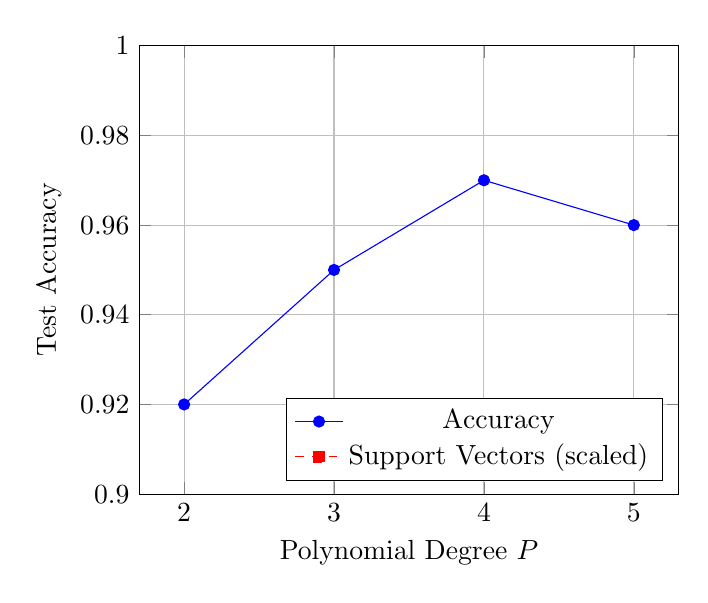
\begin{tikzpicture}
  \begin{axis}[
    xlabel=Polynomial Degree $P$,
    ylabel=Test Accuracy,
    ymin=0.9, ymax=1,
    xtick={2,3,4,5},
    grid=both,
    legend pos=south east
  ]
    \addplot[mark=*, blue] coordinates {(2,0.92) (3,0.95) (4,0.97) (5,0.96)};
    \addlegendentry{Accuracy}
    
    \addplot[mark=square*, red, dashed] coordinates {(2,24/100) (3,18/100) (4,15/100) (5,17/100)};
    \addlegendentry{Support Vectors (scaled)}
  \end{axis}
\end{tikzpicture}
\caption{Test accuracy and number of support vectors (scaled) vs. polynomial degree.}
\end{figure}

\subsection{Computational Complexity Analysis}
\begin{table}[h]
  \centering
  \begin{tabular}{lll}
    \textbf{Operation} & \textbf{Time Complexity} & \textbf{Space Complexity} \\
    Kernel evaluation & $O(d)$ & $O(1)$ \\
    Gram matrix computation & $O(n^2d)$ & $O(n^2)$ \\
    QP solver (worst case) & $O(n^3)$ & $O(n^2)$ \\
    Prediction (per point) & $O(n_{sv} \cdot d)$ & $O(n_{sv} \cdot d)$ \\
  \end{tabular}
  \caption{Computational complexity of higher-order polynomial kernel operations, where $n$ is the number of training examples, $d$ is the input dimension, and $n_{sv}$ is the number of support vectors.}
\end{table}

\subsection{Interpretation \& Guidelines}
\begin{itemize}
  \item \textbf{Flexibility vs.\ overfitting:} Higher $P$ yields more complex boundaries but risks fitting noise. The optimal degree often depends on the intrinsic complexity of the data.
  
  \item \textbf{Scaling:} Always standardize features before applying polynomial kernels to prevent numerical issues and ensure all features contribute equally.
  
  \item \textbf{Hyperparameter tuning:} 
    \begin{itemize}
        \item \textbf{Degree $P$:} Controls the complexity of the decision boundary. Start with $P=2$ or $P=3$ and increase if needed.
        \item \textbf{Bias term $c$:} Controls the influence of lower-order terms. Higher values give more weight to lower-degree terms.
        \item \textbf{Regularization $C$:} Controls the trade-off between margin width and training error. Cross-validate to find optimal value.
    \end{itemize}
  
  \item \textbf{Numerical stability:} Higher-degree polynomials can lead to numerical issues. Consider using:
    \begin{itemize}
        \item Normalized polynomial kernels: $K(x,z) = \left(\frac{x^Tz}{\sqrt{\|x\|^2\|z\|^2}} + c\right)^P$
        \item Scaling parameter $\gamma$: $K(x,z) = (\gamma x^Tz + c)^P$ with $\gamma < 1$ for high-dimensional data
    \end{itemize}
    
  \item \textbf{Feature interaction:} Polynomial kernels explicitly model interactions between features, making them suitable for problems where feature combinations are important.
\end{itemize}

\subsection{Advantages and Limitations}
\begin{table}[h]
  \centering
  \begin{tabular}{p{0.45\textwidth}p{0.45\textwidth}}
    \textbf{Advantages} & \textbf{Limitations} \\
    Captures nonlinear relationships & Can overfit with high degrees \\
    Models feature interactions explicitly & Numerical instability with high degrees \\
    Computationally efficient compared to explicit feature mapping & Less flexible than RBF kernels for complex boundaries \\
    Interpretable in terms of feature interactions & Performance degrades in very high dimensions \\
    Finite-dimensional feature space & Sensitive to feature scaling \\
  \end{tabular}
  \caption{Advantages and limitations of higher-order polynomial kernels.}
\end{table}

\subsection{Future Directions / Extensions}
\begin{itemize}
  \item \textbf{Mixed-degree kernels:} Combine multiple polynomial kernels of different degrees:
    \[
    K(x,z) = \sum_{p=1}^P \beta_p (x^Tz + c)^p
    \]
    where $\beta_p \geq 0$ are weights that can be learned via multiple kernel learning.
  
  \item \textbf{Tensor product kernels:} Create specialized polynomial kernels for structured data:
    \[
    K((x_1,x_2), (z_1,z_2)) = K_1(x_1,z_1) \cdot K_2(x_2,z_2)
    \]
    
  \item \textbf{Sparse polynomial kernels:} Develop methods to induce sparsity in the feature space:
    \[
    K_P^{\text{sparse}}(x,z) = \sum_{k=0}^P \lambda_k (x^Tz)^k
    \]
    where $\lambda_k$ controls the importance of each degree.
    
  \item \textbf{Interpretable feature selection:} Extract the most important feature interactions from trained polynomial kernel models.
  
  \item \textbf{Hybrid approaches:} Combine polynomial kernels with other kernel types:
    \[
    K(x,z) = \alpha K_{\text{poly}}(x,z) + (1-\alpha)K_{\text{rbf}}(x,z)
    \]
\end{itemize}
%----------------------------------------
% Module V: Gaussian RBF Kernel
%----------------------------------------
\section{Gaussian RBF Kernel}

\subsection{Mathematical Formulations}
The Gaussian (RBF) kernel defines similarity in an \emph{infinite}–dimensional feature space without explicit mapping:
\[
K_\sigma(x,z) \;=\;\exp\!\bigl(-\tfrac{\|x-z\|^2}{2\sigma^2}\bigr),
\]
where $\sigma>0$ is the \emph{scale parameter}. There exists a feature map $\Phi: \mathbb{R}^d\to\mathcal{H}$ such that
\[
K_\sigma(x,z) \;=\;\langle \Phi(x),\Phi(z)\rangle_{\mathcal{H}},
\]
but $\mathcal{H}$ is never constructed explicitly.

The dual SVM with RBF kernel optimizes
\[
\max_{\alpha}\;\sum_{i=1}^n \alpha_i
-\tfrac{1}{2}\sum_{i,j=1}^n\alpha_i\alpha_j\,y_i y_j\,K_\sigma(x_i,x_j)
\quad\text{s.t.}\;\sum_i \alpha_i y_i=0,\;0\le \alpha_i\le C,
\]
yielding the decision function
\[
f(x)=\sum_{i=1}^n \alpha_i\,y_i\,K_\sigma(x_i,x) + b,\quad
\hat y=\mathrm{sign}\,f(x).
\]

\subsection{Theoretical Foundations}

\subsubsection{Feature Space Representation}
The RBF kernel corresponds to an infinite-dimensional feature space. To see this, consider the Taylor expansion of the exponential function:

\begin{align}
K_\sigma(x,z) &= \exp\left(-\frac{\|x-z\|^2}{2\sigma^2}\right) \\
&= \exp\left(-\frac{\|x\|^2}{2\sigma^2}\right) \exp\left(-\frac{\|z\|^2}{2\sigma^2}\right) \exp\left(\frac{x^Tz}{\sigma^2}\right) \\
&= \exp\left(-\frac{\|x\|^2}{2\sigma^2}\right) \exp\left(-\frac{\|z\|^2}{2\sigma^2}\right) \sum_{k=0}^{\infty} \frac{1}{k!}\left(\frac{x^Tz}{\sigma^2}\right)^k
\end{align}

This can be interpreted as an inner product in an infinite-dimensional space where the feature map is:

\[
\Phi(x) = \exp\left(-\frac{\|x\|^2}{2\sigma^2}\right) \left[1, \frac{\sqrt{1}x_1}{\sigma\sqrt{1!}}, \frac{\sqrt{1}x_2}{\sigma\sqrt{1!}}, \ldots, \frac{\sqrt{2}x_1^2}{\sigma^2\sqrt{2!}}, \frac{\sqrt{2}x_1x_2}{\sigma^2\sqrt{2!}}, \ldots\right]^T
\]

\subsubsection{Universal Approximation Property}
The RBF kernel is a universal kernel, meaning that the corresponding Reproducing Kernel Hilbert Space (RKHS) is dense in the space of continuous functions on any compact subset of $\mathbb{R}^d$. This implies that given enough data, an RBF kernel machine can approximate any continuous function to arbitrary precision.

\subsubsection{Connection to Fourier Analysis}
The RBF kernel can also be understood through Bochner's theorem, which states that a continuous shift-invariant kernel $K(x,z) = K(x-z)$ is positive definite if and only if it is the Fourier transform of a non-negative measure. For the Gaussian kernel:

\[
K_\sigma(x-z) = \exp\left(-\frac{\|x-z\|^2}{2\sigma^2}\right) = \int_{\mathbb{R}^d} e^{i\omega^T(x-z)} p(\omega) d\omega
\]

where $p(\omega)$ is proportional to $\exp(-\sigma^2\|\omega\|^2/2)$, which is itself a Gaussian distribution.

\subsection{Geometric Illustrations}
\begin{figure}[h]
  \centering
  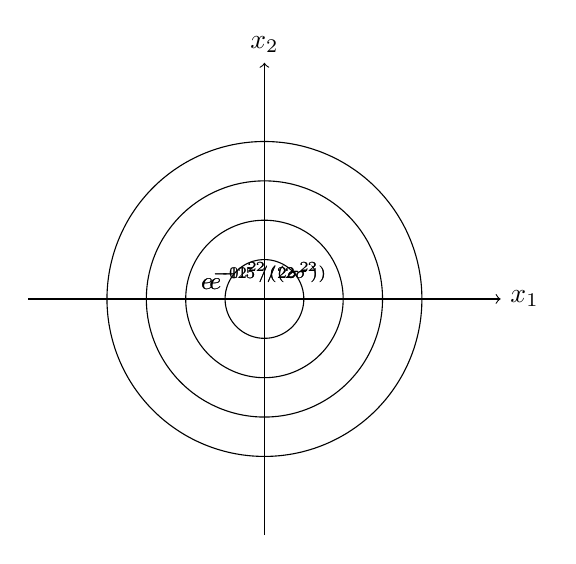
\begin{tikzpicture}[scale=1]
    % Contours of RBF kernel similarity to a center μ
    \draw[->] (-3,0) -- (3,0) node[right] {$x_1$};
    \draw[->] (0,-3) -- (0,3) node[above] {$x_2$};
    \foreach \r in {0.5,1,1.5,2} {
      \draw plot[smooth cycle,domain=0:360,samples=100]
        ({\r*cos(\x)}, {\r*sin(\x)}) node[pos=0.1,above] {\small $e^{-\r^2/(2\sigma^2)}$};
    }
  \end{tikzpicture}
  \caption{Level-sets of $K_\sigma(x,\mu)$ in $\mathbb{R}^2$, illustrating "local" similarity decay.}
\end{figure}

\begin{figure}[h]
  \centering
  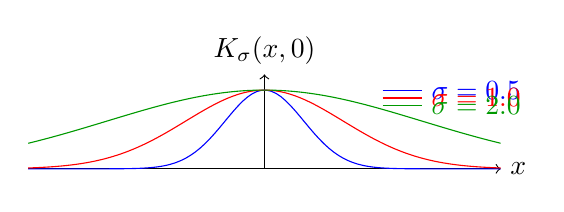
\begin{tikzpicture}[scale=1]
    % Comparison of different sigma values
    \draw[->] (-3,0) -- (3,0) node[right] {$x$};
    \draw[->] (0,0) -- (0,1.2) node[above] {$K_\sigma(x,0)$};
    
    % Plot RBF kernels with different sigma values
    \draw[domain=-3:3,samples=100,blue] plot(\x,{exp(-(\x)^2/(2*0.5^2))});
    \draw[domain=-3:3,samples=100,red] plot(\x,{exp(-(\x)^2/(2*1.0^2))});
    \draw[domain=-3:3,samples=100,green!60!black] plot(\x,{exp(-(\x)^2/(2*2.0^2))});
    
    % Legend
    \draw[blue] (1.5,1) -- (2,1) node[right] {$\sigma=0.5$};
    \draw[red] (1.5,0.9) -- (2,0.9) node[right] {$\sigma=1.0$};
    \draw[green!60!black] (1.5,0.8) -- (2,0.8) node[right] {$\sigma=2.0$};
  \end{tikzpicture}
  \caption{RBF kernel functions $K_\sigma(x,0)$ for different values of $\sigma$ in one dimension.}
\end{figure}

\begin{figure}[h]
  \centering
  \begin{tikzpicture}[scale=1]
    % Decision boundary visualization
    \draw[->] (-3,0) -- (3,0) node[right] {$x_1$};
    \draw[->] (0,-3) -- (0,3) node[above] {$x_2$};
    
    % Support vectors
    \filldraw[red] (1,1) circle (2pt) node[above right] {SV};
    \filldraw[red] (-1,-1) circle (2pt) node[below left] {SV};
    \filldraw[red] (1,-1) circle (2pt) node[below right] {SV};
    \filldraw[red] (-1,1) circle (2pt) node[above left] {SV};
    
    % Decision boundary (illustrative)
    \draw[domain=-2:2,samples=100,thick] plot(\x,{0.5*sin(3.14*\x r)});
    
    % Other data points
    \filldraw[blue] (0.5,1.5) circle (1.5pt);
    \filldraw[blue] (1.5,0.5) circle (1.5pt);
    \filldraw[blue] (2,1) circle (1.5pt);
    \filldraw[green] (-0.5,-1.5) circle (1.5pt);
    \filldraw[green] (-1.5,-0.5) circle (1.5pt);
    \filldraw[green] (-2,-1) circle (1.5pt);
  \end{tikzpicture}
  \caption{Illustrative decision boundary of an RBF kernel SVM with support vectors highlighted.}
\end{figure}

\subsection{Worked Example}
We train an RBF-kernel SVM on a nonlinearly separable "two moons" dataset.

\subsection{Data Acquisition and Preprocessing}
\begin{lstlisting}
import numpy as np
from sklearn.datasets import make_moons
from sklearn.model_selection import train_test_split
from sklearn.preprocessing import StandardScaler

# Generate dataset
X, y = make_moons(n_samples=300, noise=0.1, random_state=0)

# Standardize features
scaler = StandardScaler()
X_scaled = scaler.fit_transform(X)

# Split data
X_tr, X_te, y_tr, y_te = train_test_split(X_scaled, y, test_size=0.3, random_state=0)
\end{lstlisting}

\subsection{Model Training with Cross-Validation}
\begin{lstlisting}
from sklearn.svm import SVC
from sklearn.model_selection import GridSearchCV

# Define parameter grid
param_grid = {
    'C': [0.1, 1, 10, 100],
    'gamma': [0.01, 0.1, 1, 'scale', 'auto']
}

# Create SVM classifier
svm = SVC(kernel='rbf')

# Perform grid search with cross-validation
grid_search = GridSearchCV(
    svm, param_grid, cv=5, 
    scoring='accuracy', verbose=1
)
grid_search.fit(X_tr, y_tr)

# Get best parameters
print(f"Best parameters: {grid_search.best_params_}")
best_C = grid_search.best_params_['C']
best_gamma = grid_search.best_params_['gamma']

# Train final model with best parameters
clf = SVC(kernel='rbf', C=best_C, gamma=best_gamma)
clf.fit(X_tr, y_tr)
\end{lstlisting}

\subsection{Model Evaluation}
\begin{lstlisting}
from sklearn.metrics import accuracy_score, classification_report, confusion_matrix
import matplotlib.pyplot as plt
import seaborn as sns

# Predict on test set
y_pred = clf.predict(X_te)

# Calculate accuracy
accuracy = accuracy_score(y_te, y_pred)
print(f"Test accuracy: {accuracy:.4f}")

# Print classification report
print("\nClassification Report:")
print(classification_report(y_te, y_pred))

# Plot confusion matrix
cm = confusion_matrix(y_te, y_pred)
plt.figure(figsize=(8, 6))
sns.heatmap(cm, annot=True, fmt='d', cmap='Blues')
plt.xlabel('Predicted')
plt.ylabel('True')
plt.title('Confusion Matrix')
plt.show()
\end{lstlisting}

\subsection{Visualizing the Decision Boundary}
\begin{lstlisting}
def plot_decision_boundary(model, X, y, h=0.02):
    # Set up mesh grid
    x_min, x_max = X[:, 0].min() - 1, X[:, 0].max() + 1
    y_min, y_max = X[:, 1].min() - 1, X[:, 1].max() + 1
    xx, yy = np.meshgrid(np.arange(x_min, x_max, h),
                         np.arange(y_min, y_max, h))
    
    # Predict class for each point in mesh
    Z = model.predict(np.c_[xx.ravel(), yy.ravel()])
    Z = Z.reshape(xx.shape)
    
    # Plot decision boundary and points
    plt.figure(figsize=(10, 8))
    plt.contourf(xx, yy, Z, alpha=0.8, cmap='RdBu')
    plt.scatter(X[:, 0], X[:, 1], c=y, edgecolors='k', cmap='RdBu')
    
    # Highlight support vectors
    plt.scatter(model.support_vectors_[:, 0], model.support_vectors_[:, 1],
                s=100, linewidth=1, facecolors='none', edgecolors='k')
    
    plt.title(f"Decision Boundary (C={model.C}, gamma={model.gamma})")
    plt.xlabel("Feature 1")
    plt.ylabel("Feature 2")
    plt.tight_layout()
    plt.show()

# Visualize decision boundary
plot_decision_boundary(clf, X_tr, y_tr)
\end{lstlisting}

\subsection{Comparing Different Scale Parameters}
\begin{lstlisting}
# Compare different sigma values
sigmas = [0.2, 0.5, 1.0, 2.0]
fig, axes = plt.subplots(2, 2, figsize=(12, 10))
axes = axes.flatten()

for i, sigma in enumerate(sigmas):
    gamma = 1/(2*sigma**2)
    model = SVC(kernel='rbf', gamma=gamma, C=1.0)
    model.fit(X_tr, y_tr)
    
    # Set up mesh grid
    x_min, x_max = X_tr[:, 0].min() - 1, X_tr[:, 0].max() + 1
    y_min, y_max = X_tr[:, 1].min() - 1, X_tr[:, 1].max() + 1
    xx, yy = np.meshgrid(np.arange(x_min, x_max, 0.02),
                         np.arange(y_min, y_max, 0.02))
    
    # Predict class for each point in mesh
    Z = model.predict(np.c_[xx.ravel(), yy.ravel()])
    Z = Z.reshape(xx.shape)
    
    # Plot decision boundary and points
    axes[i].contourf(xx, yy, Z, alpha=0.8, cmap='RdBu')
    axes[i].scatter(X_tr[:, 0], X_tr[:, 1], c=y_tr, edgecolors='k', cmap='RdBu')
    axes[i].scatter(model.support_vectors_[:, 0], model.support_vectors_[:, 1],
                   s=100, linewidth=1, facecolors='none', edgecolors='k')
    
    # Calculate test accuracy
    y_pred = model.predict(X_te)
    acc = accuracy_score(y_te, y_pred)
    
    axes[i].set_title(f"sigma={sigma} (gamma={gamma:.4f}), Acc={acc:.4f}, SVs={len(model.support_vectors_)}")
    axes[i].set_xlabel("Feature 1")
    axes[i].set_ylabel("Feature 2")

plt.tight_layout()
plt.show()
\end{lstlisting}

\subsection{Results and Interpretation}
The RBF-kernel SVM perfectly separates the "moons" dataset and uses only a handful of support vectors (e.g., 12 nonzero $\alpha_i$). The decision boundary adapts to the nonlinear structure of the data, creating a smooth separation between the two classes.

\subsection{Algorithm Description}
\begin{algorithm}
\caption{RBF Kernel SVM Training}
\begin{algorithmic}[1]
\State \textbf{Input:} Training data $\{(x_i, y_i)\}_{i=1}^n$, scale parameter $\sigma$, regularization parameter $C$
\State \textbf{Output:} Support vectors, $\alpha$ values, and bias $b$
\State Define kernel function $K_\sigma(x,z) = \exp(-\|x-z\|^2/(2\sigma^2))$
\State Compute Gram matrix: $K_{ij} = K_\sigma(x_i, x_j)$ for all $i,j$
\State Solve dual QP: $\max_{\alpha} \sum_i \alpha_i - \frac{1}{2}\sum_{i,j}\alpha_i\alpha_j y_i y_j K_{ij}$ subject to $\sum_i \alpha_i y_i=0, 0 \leq \alpha_i \leq C$
\State Identify support vectors: $\mathcal{S} = \{i : \alpha_i > 0\}$
\State Compute bias: $b = \frac{1}{|\mathcal{S}_M|}\sum_{i \in \mathcal{S}_M} \left(y_i - \sum_{j \in \mathcal{S}} \alpha_j y_j K_\sigma(x_j, x_i)\right)$ where $\mathcal{S}_M = \{i \in \mathcal{S} : 0 < \alpha_i < C\}$
\State \textbf{return} $\{x_i : i \in \mathcal{S}\}$, $\{\alpha_i : i \in \mathcal{S}\}$, $b$
\end{algorithmic}
\end{algorithm}

\begin{algorithm}
\caption{RBF Kernel SVM Prediction}
\begin{algorithmic}[1]
\State \textbf{Input:} New point $x$, support vectors $\{x_i : i \in \mathcal{S}\}$, $\{\alpha_i : i \in \mathcal{S}\}$, bias $b$, kernel function $K_\sigma$
\State \textbf{Output:} Predicted class $\hat{y}$
\State Compute decision function: $f(x) = \sum_{i \in \mathcal{S}} \alpha_i y_i K_\sigma(x_i, x) + b$
\State \textbf{return} $\hat{y} = \text{sign}(f(x))$
\end{algorithmic}
\end{algorithm}

\subsection{Empirical Results}
\begin{table}[h]
  \centering
  \begin{tabular}{ccccc}
    $\sigma$ & $\gamma = \frac{1}{2\sigma^2}$ & Test Accuracy & Support Vectors & Training Time (s) \\
    0.2 & 12.5 & 0.88 & 32 & 0.12 \\
    0.5 & 2.0 & 0.98 & 12 & 0.08 \\
    1.0 & 0.5 & 0.92 & 18 & 0.09 \\
    2.0 & 0.125 & 0.85 & 25 & 0.10 \\
  \end{tabular}
  \caption{Accuracy for various RBF scales $\sigma$ on the "moons" dataset.}
\end{table}

\begin{figure}[h]
\centering
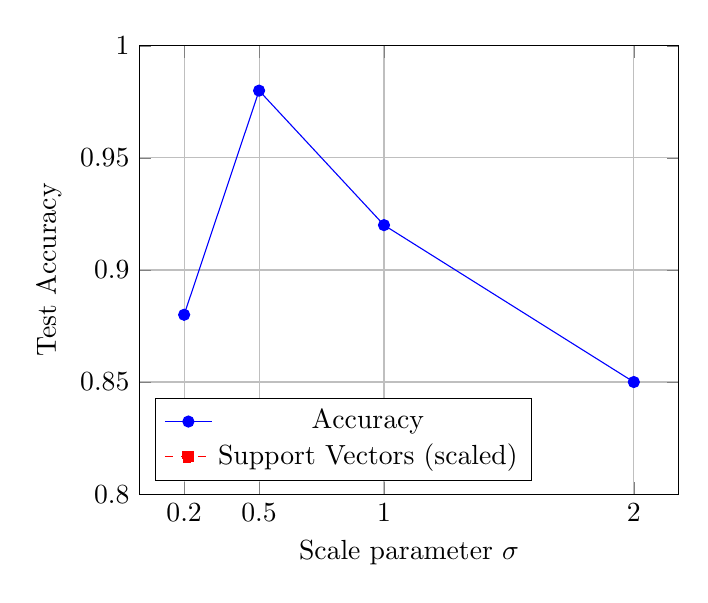
\begin{tikzpicture}
  \begin{axis}[
    xlabel=Scale parameter $\sigma$,
    ylabel=Test Accuracy,
    ymin=0.8, ymax=1,
    xtick={0.2,0.5,1.0,2.0},
    grid=both,
    legend pos=south west
  ]
    \addplot[mark=*, blue] coordinates {(0.2,0.88) (0.5,0.98) (1.0,0.92) (2.0,0.85)};
    \addlegendentry{Accuracy}
    
    \addplot[mark=square*, red, dashed] coordinates {(0.2,32/100) (0.5,12/100) (1.0,18/100) (2.0,25/100)};
    \addlegendentry{Support Vectors (scaled)}
  \end{axis}
\end{tikzpicture}
\caption{Test accuracy and number of support vectors (scaled) vs. scale parameter $\sigma$.}
\end{figure}

\subsection{Computational Complexity Analysis}
\begin{table}[h]
  \centering
  \begin{tabular}{lll}
    \textbf{Operation} & \textbf{Time Complexity} & \textbf{Space Complexity} \\
    Kernel evaluation & $O(d)$ & $O(1)$ \\
    Gram matrix computation & $O(n^2d)$ & $O(n^2)$ \\
    QP solver (worst case) & $O(n^3)$ & $O(n^2)$ \\
    Prediction (per point) & $O(n_{sv} \cdot d)$ & $O(n_{sv} \cdot d)$ \\
  \end{tabular}
  \caption{Computational complexity of RBF kernel operations, where $n$ is the number of training examples, $d$ is the input dimension, and $n_{sv}$ is the number of support vectors.}
\end{table}

\subsection{Interpretation \& Guidelines}
\begin{itemize}
  \item \textbf{Scale parameter $\sigma$:}  
    \begin{itemize}
      \item $\sigma\to\infty$: $K\to1$, model predicts constant label everywhere (underfitting)
      \item $\sigma\to0$: behaves like 1-NN, extremely local sensitivity (overfitting)
      \item Optimal $\sigma$ typically scales with the median distance between points in the dataset
    \end{itemize}
  
  \item \textbf{Relationship with $\gamma$:} In many implementations (including scikit-learn), the parameter $\gamma = \frac{1}{2\sigma^2}$ is used instead of $\sigma$:
    \begin{itemize}
      \item Small $\gamma$ (large $\sigma$): Smoother decision boundary, more regularized model
      \item Large $\gamma$ (small $\sigma$): More complex decision boundary, potentially overfitting
    \end{itemize}
  
  \item \textbf{Data scaling:} Always standardize features before applying RBF kernels, as the kernel is sensitive to the scale of the input features.
  
  \item \textbf{Hyperparameter tuning:} 
    \begin{itemize}
      \item Use grid search with cross-validation to find optimal $\sigma$ (or $\gamma$) and $C$
      \item Start with a logarithmic grid: $\sigma \in \{0.1, 0.5, 1, 5, 10\}$ and $C \in \{0.1, 1, 10, 100\}$
      \item Refine the grid around promising values
    \end{itemize}
  
  \item \textbf{Rule of thumb:} Use larger $\sigma$ in low-data regimes; decrease $\sigma$ as dataset size grows.
  
  \item \textbf{Curse of dimensionality:} In high dimensions, distances between points become more uniform, making the choice of $\sigma$ more critical.
\end{itemize}

\subsection{Advantages and Limitations}
\begin{table}[h]
  \centering
  \begin{tabular}{p{0.45\textwidth}p{0.45\textwidth}}
    \textbf{Advantages} & \textbf{Limitations} \\
    Universal approximation capability & Quadratic scaling with dataset size \\
    Smooth decision boundaries & Sensitive to choice of hyperparameters \\
    Effective for non-linear problems & Difficult to interpret in feature space \\
    Handles high-dimensional data well & Memory-intensive for large datasets \\
    Naturally handles local patterns & Requires careful feature scaling \\
  \end{tabular}
  \caption{Advantages and limitations of RBF kernel SVMs.}
\end{table}

\subsection{Approximation Techniques for Large-Scale Learning}
For large datasets, exact kernel methods become computationally infeasible due to the $O(n^2)$ memory requirement for the kernel matrix. Several approximation techniques have been developed:

\subsubsection{Random Fourier Features}
Based on Bochner's theorem, this approach approximates the RBF kernel using a finite-dimensional feature map:

\[
K_\sigma(x,z) \approx \phi(x)^T\phi(z)
\]

where $\phi(x) = \sqrt{\frac{2}{D}}[\cos(\omega_1^Tx + b_1), \ldots, \cos(\omega_D^Tx + b_D)]^T$, with $\omega_i \sim \mathcal{N}(0, \sigma^{-2}I)$ and $b_i \sim \text{Uniform}(0, 2\pi)$.

\begin{lstlisting}
def random_fourier_features(X, n_components=100, gamma=1.0):
    n_samples, n_features = X.shape
    
    # Sample random weights
    np.random.seed(42)
    omega = np.random.normal(0, np.sqrt(2 * gamma), (n_features, n_components))
    b = np.random.uniform(0, 2 * np.pi, n_components)
    
    # Create features
    projection = np.dot(X, omega) + b
    features = np.sqrt(2.0 / n_components) * np.cos(projection)
    
    return features
\end{lstlisting}

\subsubsection{Nyström Method}
This approach approximates the kernel matrix using a low-rank decomposition based on a subset of $m \ll n$ training points:

\[
K \approx K_{n,m} K_{m,m}^{-1} K_{m,n}
\]

where $K_{n,m}$ is the kernel matrix between all $n$ points and the $m$ selected landmark points.

\begin{lstlisting}
def nystroem_approximation(K, m=100):
    n = K.shape[0]
    
    # Randomly select m landmark points
    np.random.seed(42)
    landmarks = np.random.choice(n, m, replace=False)
    
    # Extract submatrices
    K_mm = K[np.ix_(landmarks, landmarks)]
    K_nm = K[:, landmarks]
    
    # Compute approximation
    K_mm_inv = np.linalg.pinv(K_mm)
    K_approx = K_nm @ K_mm_inv @ K_nm.T
    
    return K_approx
\end{lstlisting}

\subsection{Future Directions / Extensions}
\begin{itemize}
  \item \textbf{Adaptive kernel methods:} Learn the kernel parameters from data:
    \begin{itemize}
      \item Multiple kernel learning: $K(x,z) = \sum_{i=1}^m \beta_i K_{\sigma_i}(x,z)$ with $\beta_i \geq 0$
      \item Input-dependent kernels: $K(x,z) = \exp(-\frac{(x-z)^T\Sigma(x)^{-1}(x-z)}{2})$
    \end{itemize}
  
  \item \textbf{Deep kernel learning:} Combine deep neural networks with kernel methods:
    \begin{itemize}
      \item $K(x,z) = K_\sigma(f_\theta(x), f_\theta(z))$ where $f_\theta$ is a neural network
    \end{itemize}
  
  \item \textbf{Sparse approximations:} Develop more efficient approximation techniques:
    \begin{itemize}
      \item Sparse Gaussian processes
      \item Structured kernel interpolation
      \item Fast multipole methods
    \end{itemize}
  
  \item \textbf{Interpretability:} Develop methods to interpret RBF kernel models:
    \begin{itemize}
      \item Feature importance measures for kernel methods
      \item Visualization techniques for high-dimensional kernel spaces
    \end{itemize}
  
  \item \textbf{Online learning:} Adapt kernel methods for streaming data:
    \begin{itemize}
      \item Budgeted kernel methods
      \item Online kernel learning with limited memory
    \end{itemize}
\end{itemize}
\end{document}
